%\graphicspath{{screenshots/}}

\section{Bedienungsanleitung}
\subsection{Hintergrundinformationen}

\paragraph{Spielinteraktion}
\subparagraph{Selektierungsvorgang}
Um einen gewuenschten Domino zu selektieren muss der Spieler auf einen der schwarzen Kaesten rechts neben dem angezeigten Domino per Mausklick auswaehlen (siehe Abbildung \pageref{fig:erstesSelektierenNaechsteBank}) und es erscheint die Zahl \emph{1} in diesem Feld. Um dem Spieler deutlich zu machen von welcher Bank, oder ob er ueberhaupt in seinem aktuellen Zug einen Domino selektieren darf, kann er nur auf der Bank welche nicht verschwommen ist einen Domino auswaehlen. Um jederzeit ablesen zu koennen welcher Spieler gerade am Zug ist gibt es hierfuer ein Feld oberhalb der Bank fuer die naechste Runde. 

\begin{figure}
	\centering
	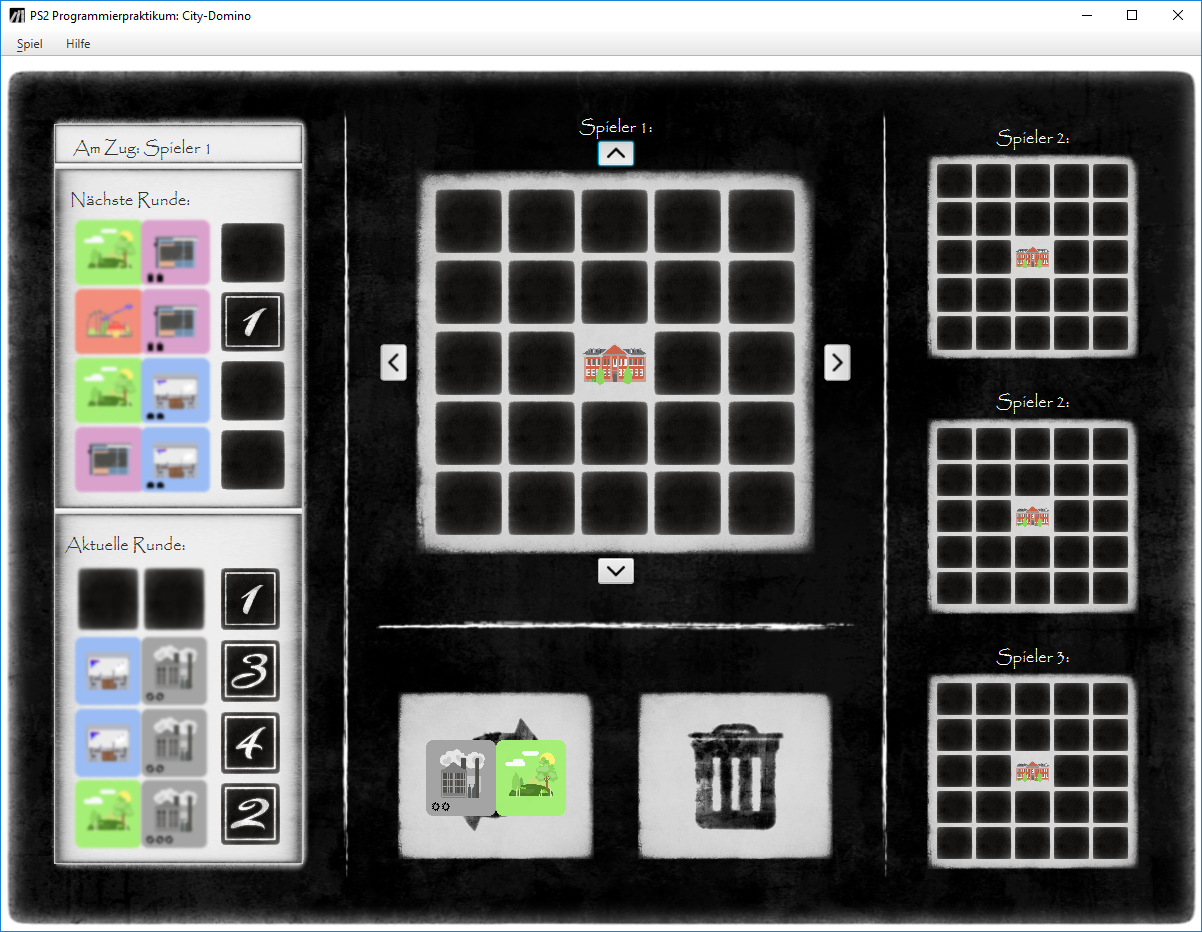
\includegraphics{screenshots/screenshot_ErstesSelektierenAufNaechsterBank}
	\caption[Erstes Selektieren]{Erstes Selektieren auf der Bank fuer die naechste Runde}
	\label{fig:erstesSelektierenNaechsteBank}
\end{figure}

\subparagraph{Justierung des Dominos}
Nachdem der Spieler erfolgreich saemtliche Selektierungsschritte auf den beiden Baenken absolviert hat, kann er seinen zuvor ausgewaehlten Domino in dem dafuer vorgesehenen Kasten drehen. Um den Domino um 90 Grad zu drehen muss der Spieler lediglich einen Mausklick auf dem Domino ausfuehren. 

\subparagraph{Positionierung auf dem Spielfeld}
Um den justierten Domino nun auf dem Feld zu platzieren zieht der Benutzer den Domino an die gewuenschte Stelle auf dem Spielfeld. Waehrend dem Ziehen faerben sich zugrunde liegenden Felder jeweils gruen, falls es moeglich sein sollte den Domino an dieser Stelle anzulegen (siehe Abbildung \pageref{fig:hovernGruen}), beziehungsweise rot, falls dies nicht der Fall sein sollte (siehe Abbildung \ref{fig:hovernRot}, fuer genauere Informationen siehe Abschnitt \ref{par:anlegeregeln}). Falls der Domino an der gewuenschten Stelle nicht passen sollte und dennoch versucht wird ihn an dieser Stelle zu platzieren, passiert nichts denn der Domino befindet sich weiterhin in dem Kasten zum justieren der Ausrichtung und es kann ein neuer Versuch gestartet werden. 

\begin{figure}
	\centering
	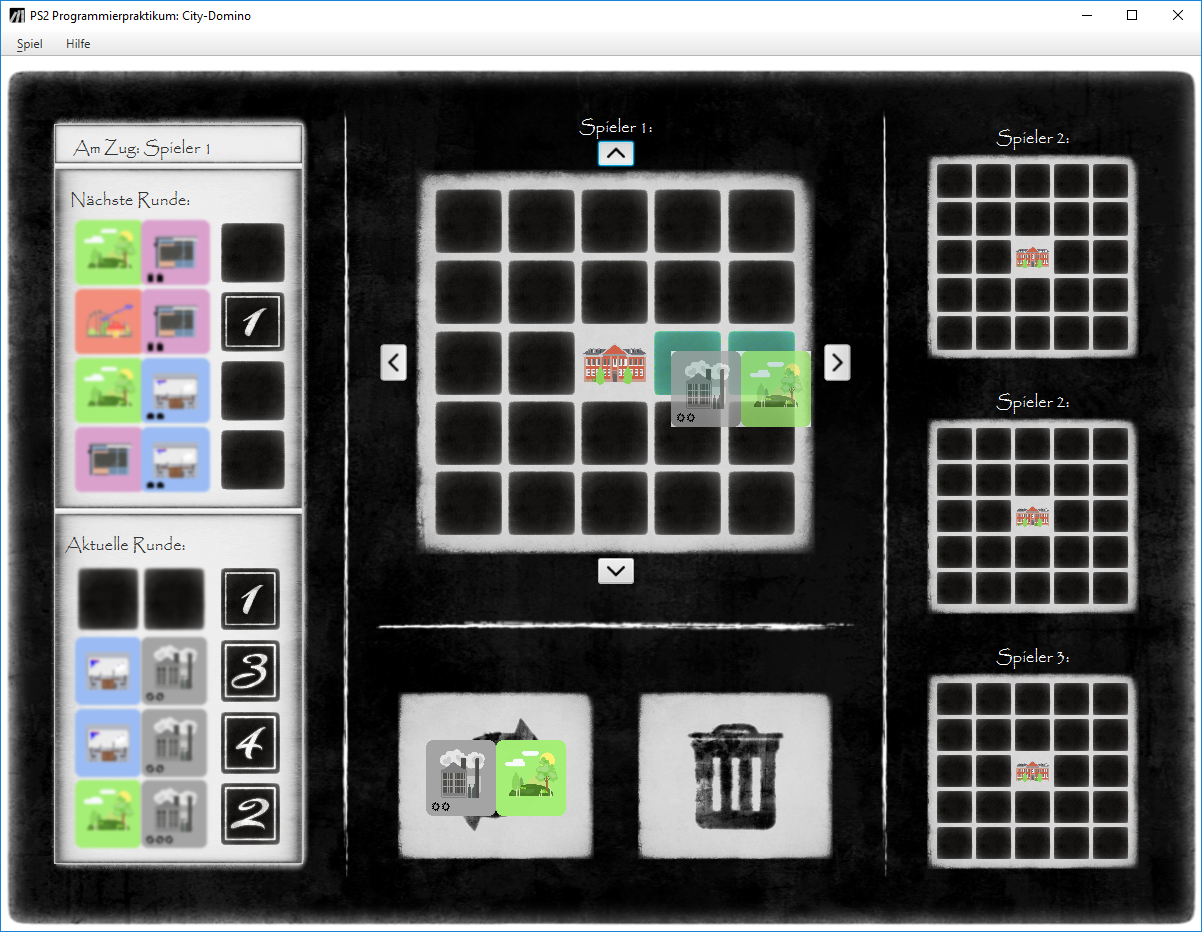
\includegraphics{screenshots/screenshot_HovernGruen}
	\caption{Schwebender Domino ueber gueltiger Position}
	\label{fig:hovernGruen}
\end{figure}

\begin{figure}
	\centering
	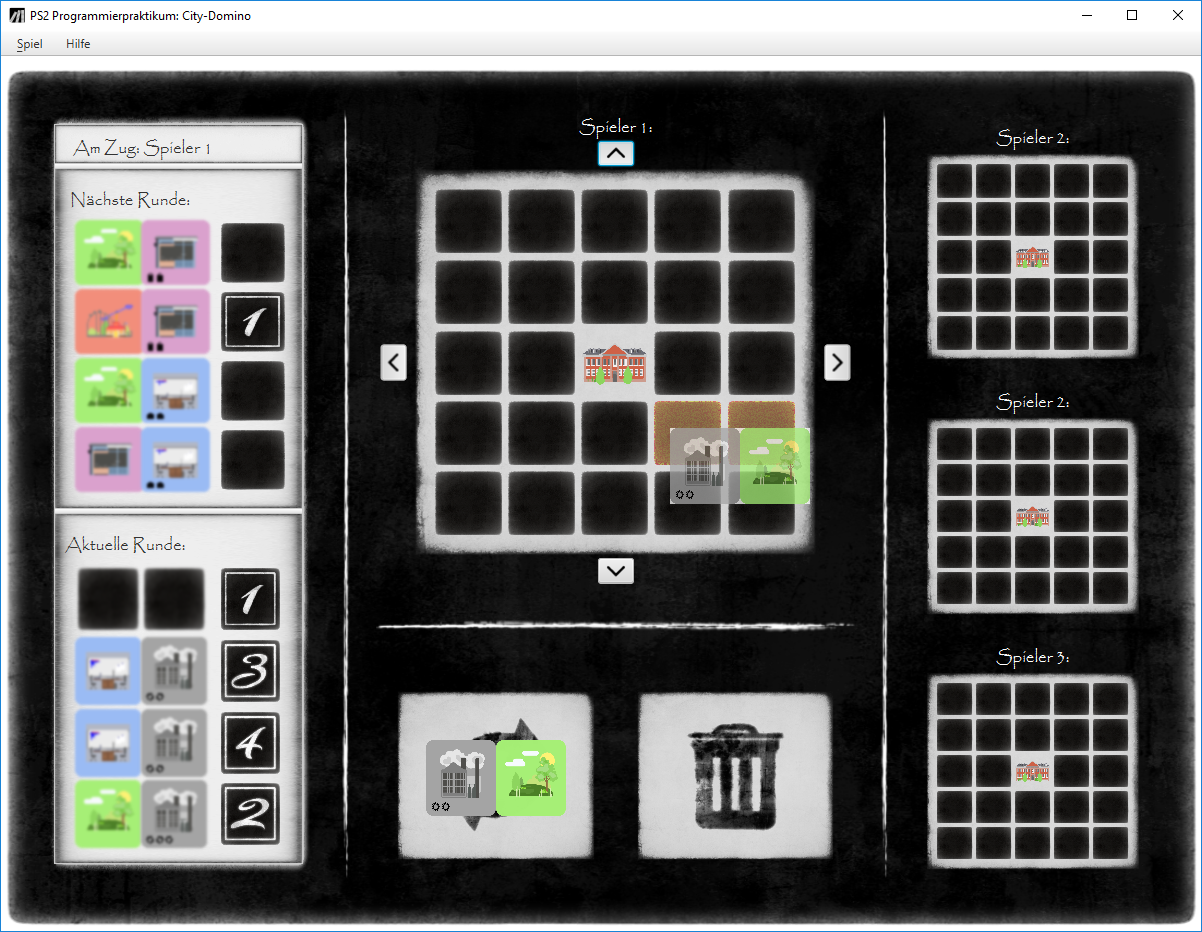
\includegraphics{screenshots/screenshot_HovernRot}
	\caption{Schwebender Domino ueber ungueltiger Position}
	\label{fig:hovernRot}
\end{figure}


\newpage

\begin{figure}
	\centering
	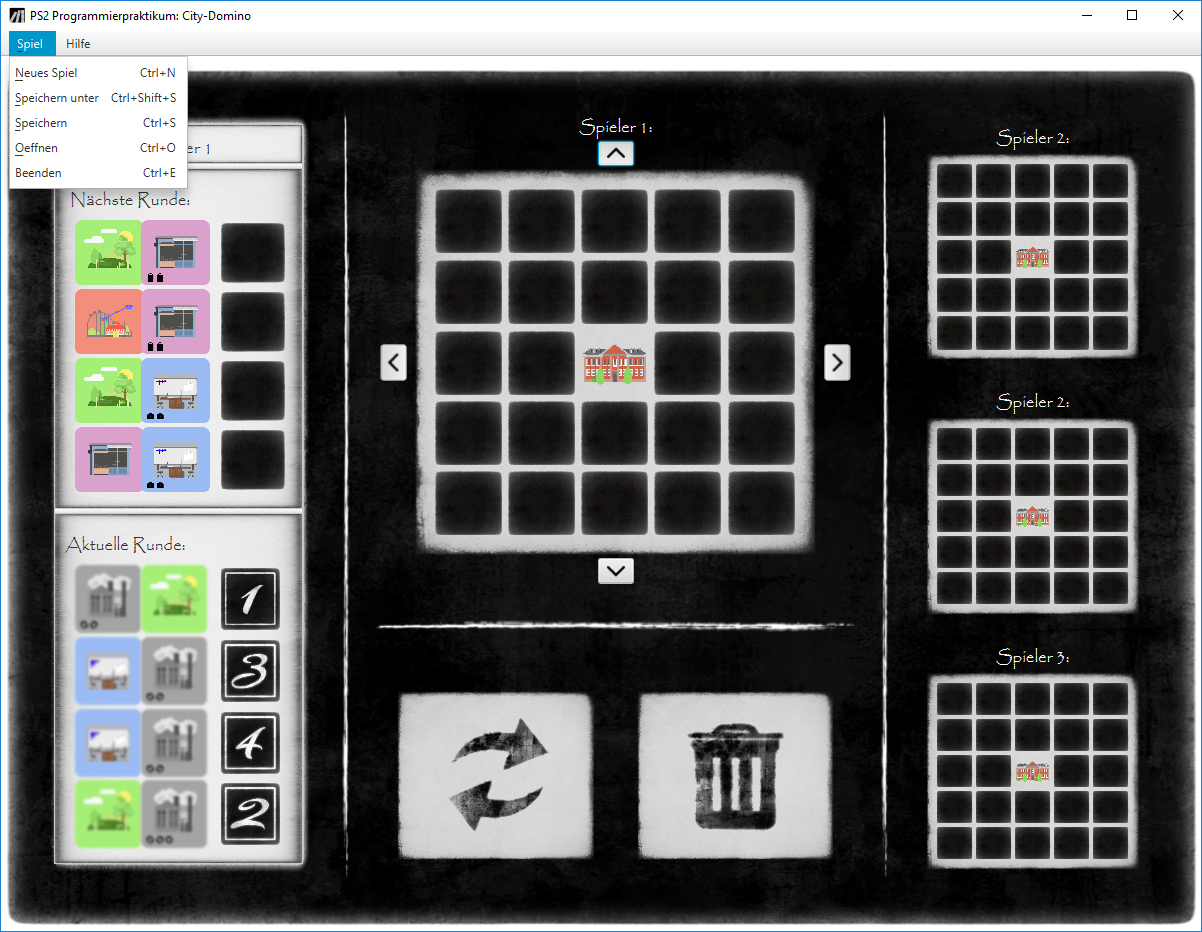
\includegraphics{screenshots/screenshot_Menue}
	\caption{Menueoptionen}
	\label{fig:menueoptionen}
\end{figure}

\paragraph{Menueinteraktion}
\subparagraph{Starten bzw. Schliessen}
Um ein neues Spiel zu starten waehlt der Benutzer den Menuepunkt "\emph{Neues Spiel}". Alternativ ist dies auch per Tastenkombination \verb|strg + N| moeglich. Um das geoffnete Fenster zu schliessen und das bestehende Spiel zu verwerfen waehlt der Benutzer den Reiter \emph{Beenden} (Tastenkombination \verb|strg + E|). Falls der Benutzer das Spiel nicht vorher gespeichert hat erscheint hierbei ein weiteres Fenster welches den Benutzer darauf hinweist und ihm die Moeglichkeit gibt dies nachzuholen (siehe folgenden Abschnitt).
\todo{Muss noch implementiert werden}

\subparagraph{Spielstand abspeichern}
Um ein Spielstand zu speichern gibt es zwei Reiter mit folgenden Moeglichkeiten.
\begin{enumerate}
	\item{Speichern: \verb|Strg + S|}
	\item{Speichern unter: \verb|Strg + Shift + S|}
\end{enumerate}
Speichern unter gibt dem Benutzer die Moeglichkeit, ausgehend vom Ablageverzeichnis den gewuenschten Speicherort anzugeben. Hierzu navigiert man mit dem gegebenen Filechooser an den gewuenschten Speicherort und gibt der abzuspeichernden Datei einen Namen, die benoetigt Dateiendung \emph{.txt} ist bereits ausgewaehlt, sodass der Benutzer seine Auswahl lediglich auf dem Feld \emph{Speichern} per Mausklick zu bestaetigen braucht (siehe Abbildung \ref{fig:filechooser}). 

Der Reiter \emph{Speichern} ermoeglicht es einen bereits gespeicherten Spielstand ohne oeffnen eines Filechoosers zu ueberschreiben. Falls der Benutzer diesen Reiter betaetigt ohne dass zuvor ein Spielstand des aktuellen Spiels abgespeichert wurde ist, oeffnet sich bei der Auswahl dieses Reiters dennoch ein Filechooser und es wird nach der Funktionsweise von \emph{Speichern unter} vorgegangen. 

\subparagraph{Oeffnen}
Aehnlich wie beim Reiter \emph{Speichern unter} wird hier ein Filechooser geoeffnet. Dieser wird jedoch dazu verwendet eine Datei auszuwaehlen um aus dieser einen Spielstand zu lesen. Falls die Datei nicht der geforderten Syntax entspricht , erscheint eine Fehlermeldung in Form eines Popup-Fensters mit dem einer groben Fehlermeldung wo der Fehler liegt(Siehe ...) 
\todo{Screenshots der Fehlermeldungen und Referenz auf Erklaerung einfuegen}
. Falls der Benutzer vor dem Oeffnen eines neuen Spielstands den alten nicht gespeichert hat wird er aehnlich wie beim Beenden darauf hingewiesen und es wird per Filechooser eine Moeglichkeit bereitgestellt dies nachzuholen. 
\todo{Muss noch implementiert werden}

\begin{figure}
	\centering
	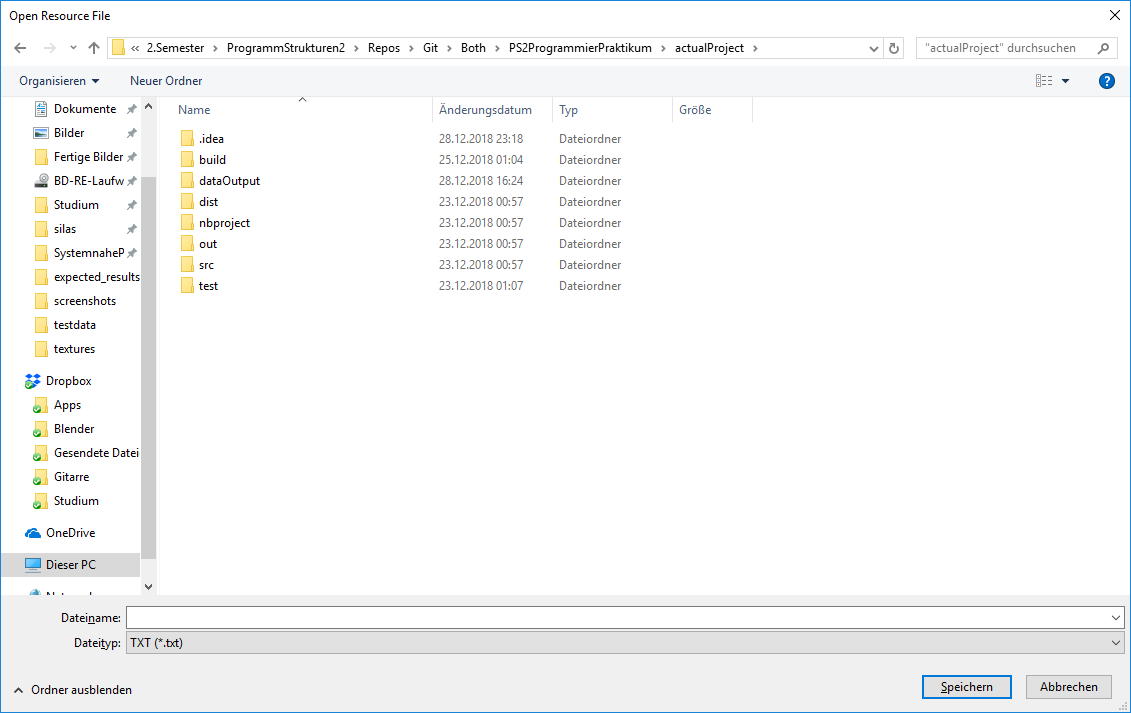
\includegraphics{screenshots/screenshot_Filechooser}
	\caption[Filechooser]{Filechooser zum Abspeichern eines Spielstandes}
	\label{fig:filechooser}
\end{figure}

\begin{figure*}
        \centering
        \begin{subfigure}[b]{0.35\textwidth}   
            \centering 
            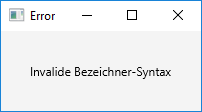
\includegraphics[width=\textwidth]{screenshots/screenshot_ErrorBezeichner}
            \caption[]%
            {{\small Bezeichner}}    
            \label{fig:mean and std of net34}
        \end{subfigure}
        \quad
        \begin{subfigure}[b]{0.35\textwidth}   
            \centering 
            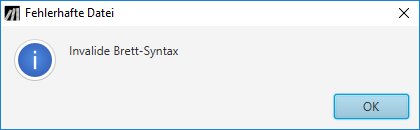
\includegraphics[width=\textwidth]{screenshots/screenshot_ErrorBrett}
            \caption[]%
            {{\small Brett}}    
            \label{fig:mean and std of net44}
        \end{subfigure}
        \vskip\baselineskip
        \begin{subfigure}[b]{0.35\textwidth}   
            \centering 
            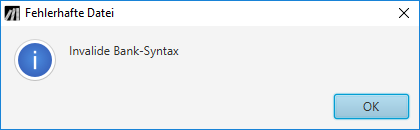
\includegraphics[width=\textwidth]{screenshots/screenshot_ErrorBank}
            \caption[]%
            {{\small Bank}}    
            \label{fig:mean and std of net34}
        \end{subfigure}
        \quad
        \begin{subfigure}[b]{0.35\textwidth}   
            \centering 
            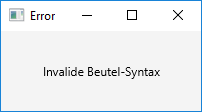
\includegraphics[width=\textwidth]{screenshots/screenshot_ErrorBeutel}
            \caption[]%
            {{\small Beutel}}    
            \label{fig:mean and std of net44}
        \end{subfigure}
        \caption
        {\small Unterschiedliche Fehlermeldungen beim Dateineinlesen} 
        \label{fig:mean and std of nets}
    \end{figure*}

\subparagraph{Hilfestellung}
Unter dem Reiter \emph{Hilfe} ist die Aufgabenstellung im Pdf-Format zu finden. Beim Auswaehlen des Menuepunktes \emph{Aufgabenstellung} oeffnet sich diese im, vom Benutzer standardmaessig genutzten, Pdf-Reader. 

\clearpage
\subsection{Programmfunktionalitaet}
Nach dem Starten des Programms ist lediglich die Bank fuer das erstmalige Selektieren der aktuellen Runde mit Dominos gefuellt (siehe Abbildung \ref{fig:spielbeginnGui}). Nun beginnt der Spieler mit dem ersten Selektieren des 
\begin{figure}
	\centering
	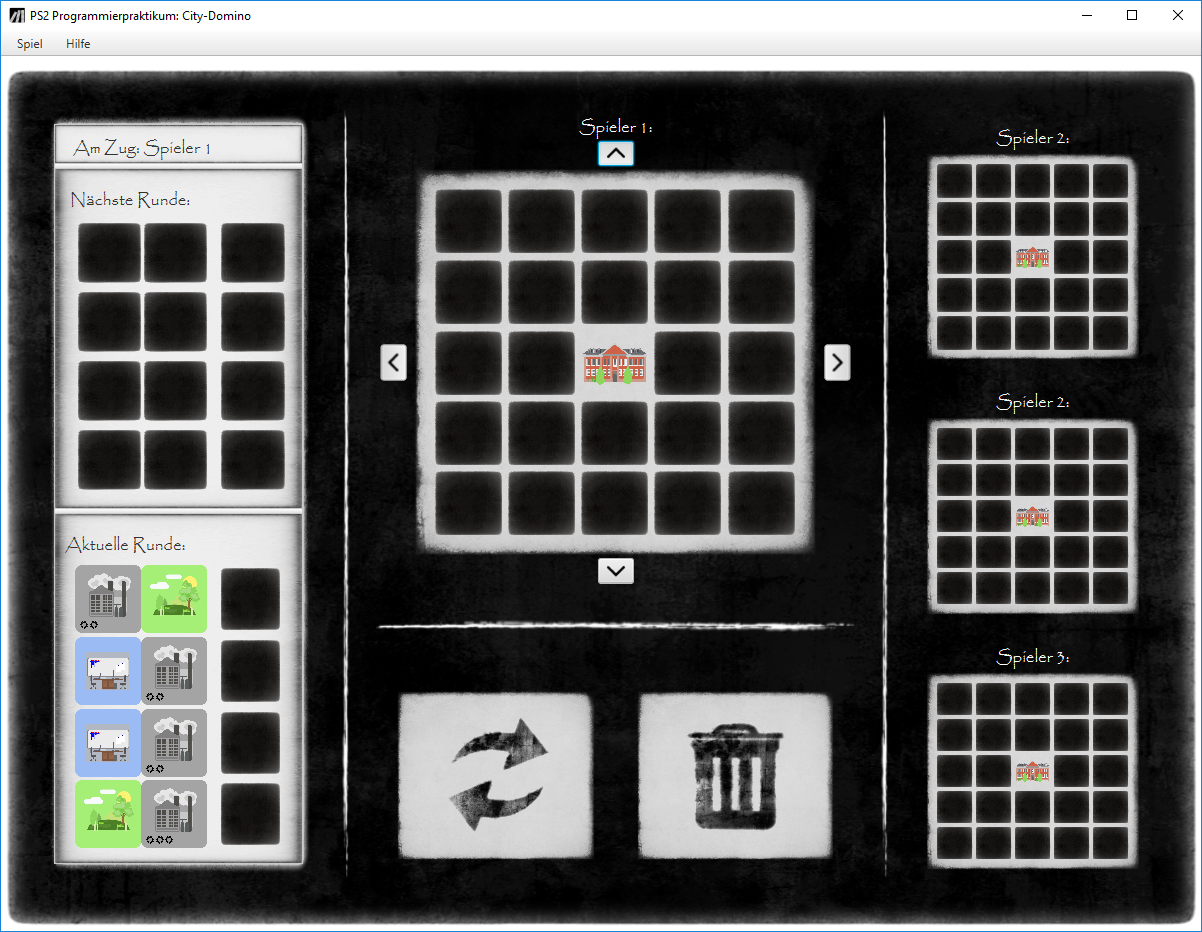
\includegraphics{screenshots/screenshot_Spielbeginn.png}
	\caption[Spielbeginn]{Spielbeginn nach Programmstart}
	\label{fig:spielbeginnGui}
\end{figure}


\label{par:anlegeregeln}